\documentclass[11pt]{article}

\usepackage[margin=1in]{geometry}
\usepackage{graphicx}
\usepackage{booktabs}
\usepackage{xcolor}
\usepackage{amsmath}
\usepackage{amssymb}
\usepackage{caption}
\usepackage{float}
% placeins unavailable on this system; with [H] floats are placed in-line, so
% a no-op \FloatBarrier suffices to keep each figure with its paragraph.
\providecommand{\FloatBarrier}{}
\usepackage[colorlinks=true,linkcolor=accent,urlcolor=accent,citecolor=accent]{hyperref}

% --- colours ---
\definecolor{accent}{RGB}{20,90,150}
\definecolor{accentlight}{RGB}{232,240,248}
\definecolor{rulegray}{RGB}{120,120,120}

% --- section heading styling: a touch of colour + a rule ---
% (titlesec/sectsty unavailable; redefine \section/\subsection via \@startsection)
\makeatletter
\renewcommand\section{\@startsection{section}{1}{\z@}%
  {-3.5ex \@plus -1ex \@minus -.2ex}%
  {2.3ex \@plus.2ex}%
  {\normalfont\Large\bfseries\color{accent}}}
\renewcommand\subsection{\@startsection{subsection}{2}{\z@}%
  {-3.25ex\@plus -1ex \@minus -.2ex}%
  {1.5ex \@plus .2ex}%
  {\normalfont\large\bfseries\color{accent}}}
\makeatother

\captionsetup{font=small,labelfont={bf,color=accent}}
\setlength{\parskip}{0.4em}
\setlength{\parindent}{0pt}

% --- headline box: framed minipage fallback (tcolorbox/mdframed unavailable) ---
\newcommand{\headlinebox}[1]{%
  \begin{center}
  \setlength{\fboxsep}{12pt}%
  \setlength{\fboxrule}{1.2pt}%
  \fcolorbox{accent}{accentlight}{%
    \begin{minipage}{0.92\textwidth}
    #1
    \end{minipage}}%
  \end{center}}

\begin{document}

% ===================== TITLE BLOCK =====================
\begin{center}
{\color{accent}\rule{\textwidth}{1.5pt}}\\[1.2em]
{\LARGE\bfseries Reproducing RS Warped Flavor \& Electroweak Constraints:\\[0.3em]
Fixed-Code Validation Against the Literature\par}
\vspace{0.8em}
{\large Minimal Randall--Sundrum, quark sector.\\
Audit fixes + reproduction of published figures.\par}
\vspace{0.7em}
{\large June 2026\par}
\vspace{0.4em}
{\color{accent}\rule{\textwidth}{1.5pt}}
\end{center}
\vspace{1em}

% ===================== INTRODUCTION =====================
\section{Introduction}

We work in a minimal Randall--Sundrum (RS) warped extra dimension; fermion mass
hierarchies come from geometric (wavefunction) localization rather than
hierarchical 5D Yukawas. An adversarial audit of our quark-sector constraint
code found six implementation errors (three blocker-level), now fixed and
dual-reviewed: \textbf{B1} the $Z\to b\bar b$ fermion-KK admixture (mistranslated
from Casagrande et al.\ 0807.4937 --- wrong sign and ${\sim}190\times$ too
large), \textbf{B2} the $\varepsilon_K$ SVD$\to$PDG rephasing ($\varepsilon_K$ was
convention-dependent), \textbf{B3} the $\Delta F=2$ $O_4/O_5$ chiral coefficients
+ state normalization, \textbf{M1} the $Z\to b\bar b$ (T010) gate, \textbf{M2} the
EW001 $\Delta T$ convention (oblique $T$ was ${\sim}6\times$ too weak), and
\textbf{M5} a tagging bug. Net effect: the headline minimal-model floor changed
qualitatively --- the old ``25--30~TeV (108~TeV at $1\sigma$) $Z\to b\bar b$
floor'' was an artifact of B1 and collapses to ${\sim}5$~TeV once corrected.

We validate the fixed code two ways. (i)~A \textbf{constrained-fit scan}: draw
bulk masses + a seed, fit the Yukawas to reproduce the measured quark masses +
CKM (a near-unique solution $\to$ a thin ``locus''). (ii)~An
\textbf{anarchic-forward scan}: draw complex $O(1)$ anarchic Yukawas, compute
observables forward, keep mass+CKM-reproducing points (the multi-decade
``cloud'' the literature uses). The papers scatter anarchic Yukawas; our
production scan fits --- so the two give very different spreads, which matters
for how floors compare to the literature.

% ===================== HEADLINE BOX =====================
\headlinebox{%
{\large\bfseries\color{accent} Headline findings}\\[0.5em]
\begin{itemize}\setlength{\itemsep}{0.35em}\leftskip-0.5em
\item The fixed code \textbf{reproduces the published RS literature} when run in
anarchic-forward mode: $\varepsilon_K$ 95\%-quantile floor = \textbf{10~TeV}
(= Bauer 0912.1625 headline), $D^0$ funnel containment rising to ${\sim}88\%$ at 10~TeV
(Gedalia), kaon $\mathrm{Im}/\mathrm{Re}(M_{12})$ = \textbf{106$\times$}
($\approx$ Blanke's ${\sim}100\times$ $\varepsilon_K$ problem), $C_{B_d}/C_{B_s}\approx1$.
\item \textbf{Minimal-model floors (corrected):} \emph{typical} anarchic floor
with current data $\approx$ \textbf{30~TeV}, set by $\varepsilon_K$ (flavor);
\emph{existence} (fine-tuned) floor $\approx$ \textbf{18--20~TeV}, set
irreducibly by \textbf{S,\,T,\,U}. $Z\to b\bar b$ no longer leads
($\approx$5~TeV).
\item Flavor constraints are \textbf{tunable} (alignment drives the NP $\to0$);
\textbf{S,\,T,\,U is irreducible} (no Yukawa freedom). This is precisely why
custodial RS exists.
\end{itemize}}

\vspace{0.6em}

% ===================== FLOOR TABLE =====================
\section{Floor summary: typical vs.\ existence}

The two scan modes give two distinct notions of a floor. The \emph{typical}
(median) floor is where the bulk of anarchic points become excluded; the
\emph{existence} (best/tuned) floor is where even the single best-aligned point
crosses the bound. Flavor constraints separate the two by orders of magnitude
(they are tunable); the oblique $S,T,U$ constraint does not (it has no Yukawa
freedom).

\begin{center}
\small
\setlength{\tabcolsep}{5pt}
\begin{tabular}{@{}llll@{}}
\toprule
\textbf{Constraint} & \textbf{Typical (median)} & \textbf{Existence (best/tuned)} & \textbf{Tunable?} \\
\midrule
$\varepsilon_K$            & ${\sim}30$~TeV (anarchic) & ${\lesssim}1$~TeV & yes (align $\mathrm{Im}\,M_{12}\!\to\!0$) \\
$\Delta m_d$ ($B_d$)       & few TeV & ${\lesssim}1$~TeV & yes \\
$\Delta m_s$ ($B_s$)       & few TeV & ${\lesssim}1$~TeV & yes \\
$D^0$                      & low & ${\lesssim}1$~TeV & yes \\
$\Delta m_K$               & low & ${\lesssim}3$~TeV & yes \\
$Z\to b\bar b$ (T010)      & ${\sim}5$~TeV & ${\sim}4.6$~TeV & no (gauge-dominated; $c_{Q_3}$ pinned by $m_t$) \\
$S,T,U$ (EW001)            & ${\sim}20$~TeV & ${\sim}18\text{--}20$~TeV & no (no Yukawa dependence) \\
\midrule
\textbf{COMBINED}          & \textbf{${\sim}30$~TeV} ($\varepsilon_K$) & \textbf{${\sim}18\text{--}20$~TeV} ($S,T,U$) & --- \\
\bottomrule
\end{tabular}
\end{center}

\FloatBarrier
\clearpage

% ===================== PER-FIGURE SECTIONS =====================
\section{Figures: reproduction and analysis}

% ---- explorer_floors ----
\subsection*{Constraint census --- our 100k minimal scan (ours only)}
\begin{figure}[H]
\centering
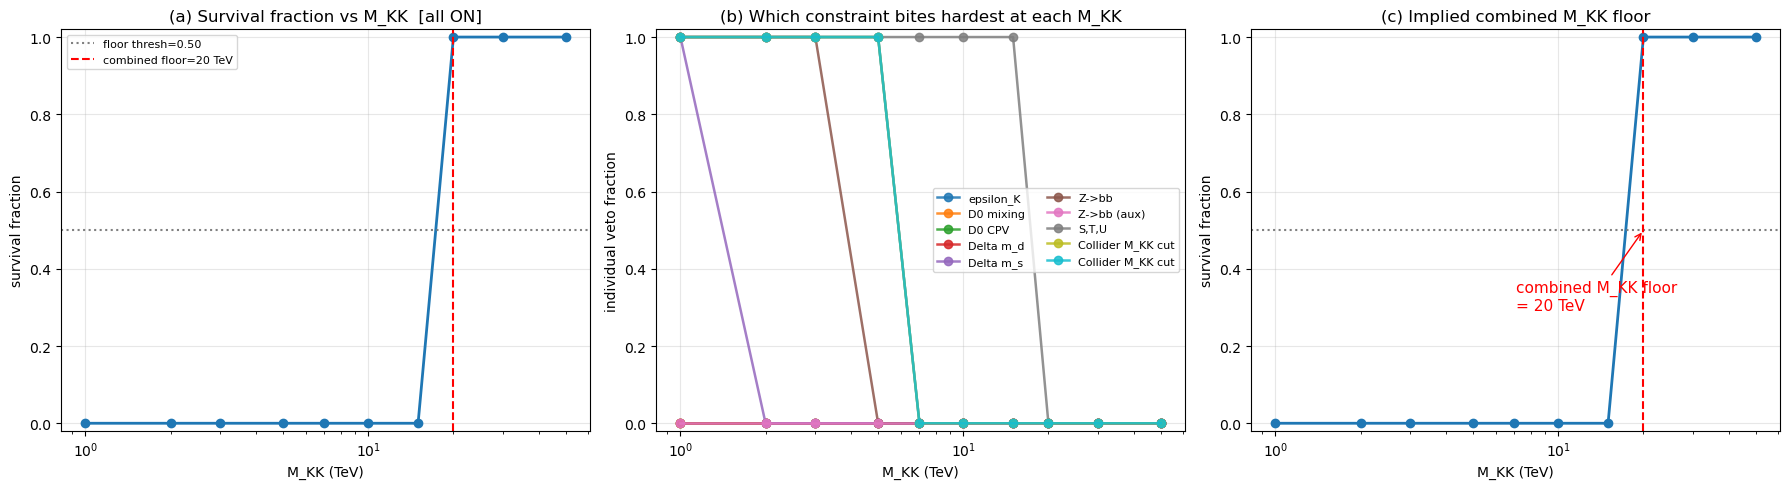
\includegraphics[width=\textwidth]{figures/fig_explorer_floors.png}
\caption{Per-constraint veto fraction vs.\ $M_{KK}$ from our 100k minimal-model
scan with all fixes in.}
\end{figure}
Per-constraint veto fraction vs.\ $M_{KK}$ from our 100k minimal-model scan with
all fixes in. The corrected ranking: \textbf{$S,T,U$ (EW001) leads at
${\sim}20$~TeV}, $\varepsilon_K$ (rigorous) at 7~TeV, \textbf{$Z\to b\bar b$
(T010) collapsed to 5~TeV} (it was the spurious ${\sim}25\text{--}30$~TeV B1
artifact), $\Delta m_s$ at 2~TeV; $D^0$/$\Delta m_d$/$Z\to b\bar b$-$A_b$ never
bind. Dropping $Z\to b\bar b$ leaves the combined floor unchanged at 20~TeV ---
concrete proof it is no longer the driver.

\FloatBarrier

% ---- STU ----
\subsection*{$S,T,U$ oblique --- Casagrande et al.\ 0807.4937, Fig.~4 \quad(paper left, ours right)}
\begin{figure}[H]
\centering
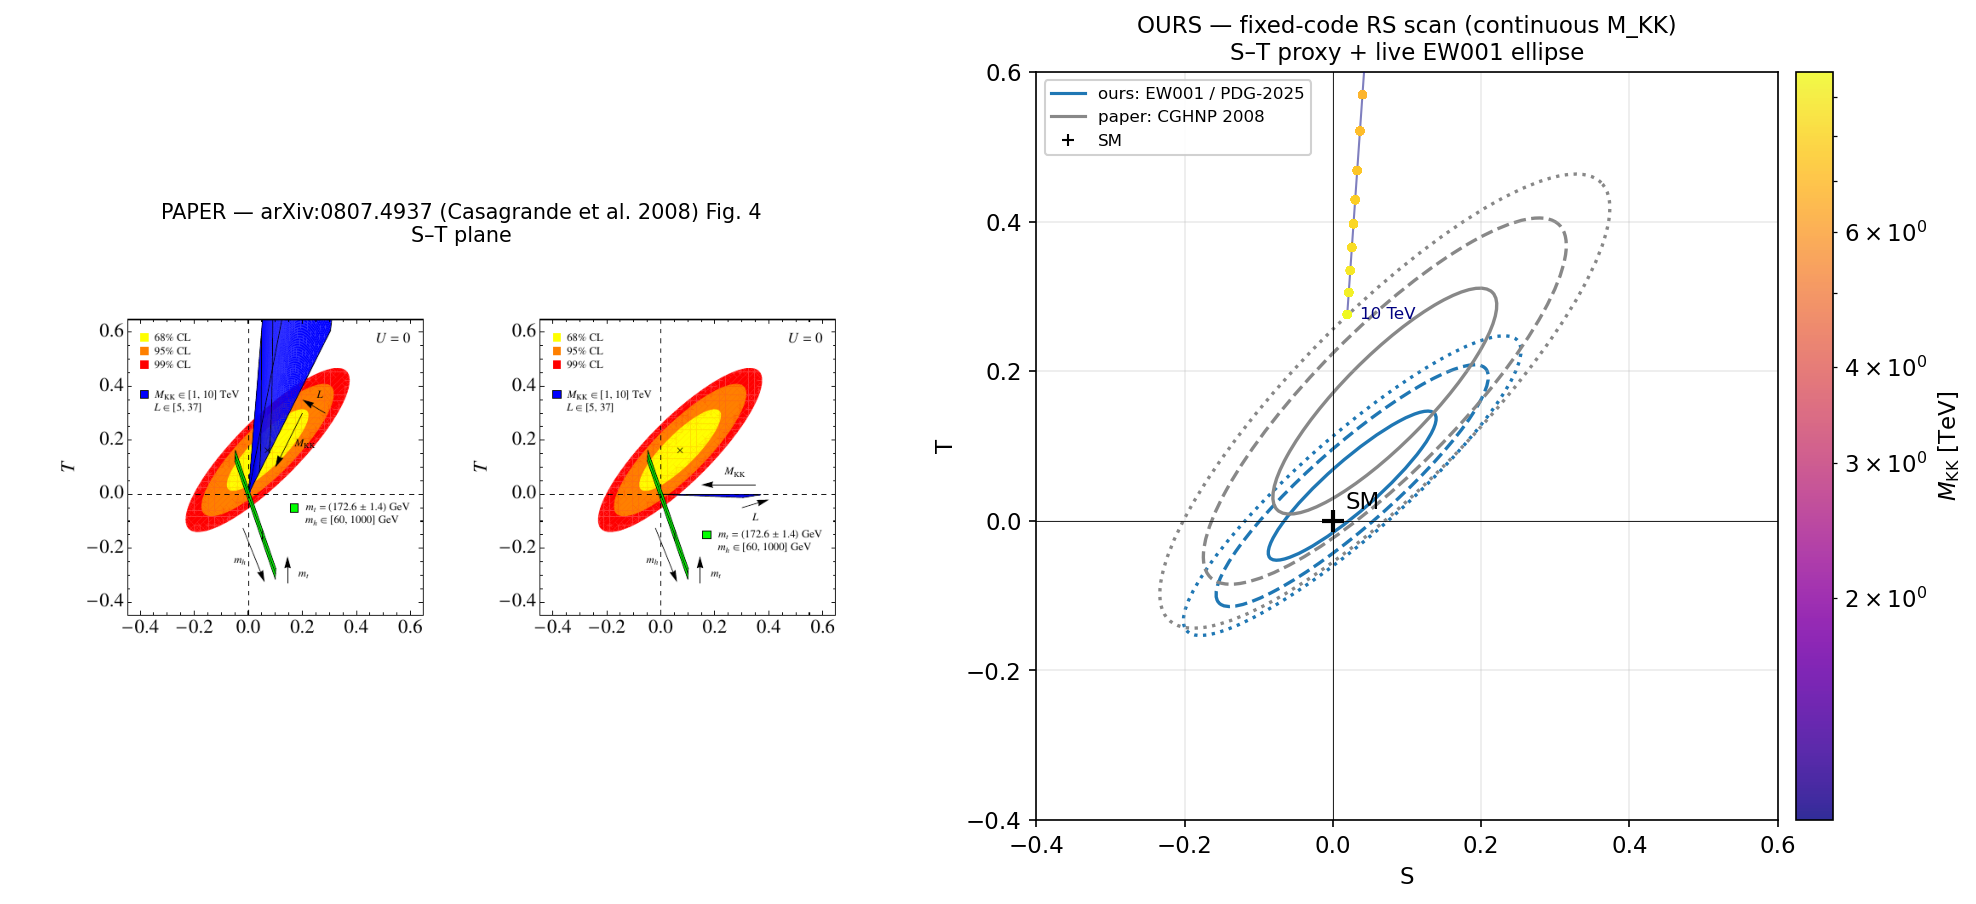
\includegraphics[width=\textwidth]{figures/fig_STU.png}
\caption{The $S$--$T$ plane: paper (left) vs.\ ours (right). Minimal RS sweeps a
wedge over $M_{KK}$ ($1\to10$~TeV) and warp volume $L$ against the CL ellipses.}
\end{figure}
The paper plots the $S$--$T$ plane with 68/95/99\% CL ellipses and the minimal-RS
``wedge'' swept over $M_{KK}$ ($1\to10$~TeV) and warp volume $L$. Minimal RS
climbs steeply in \textbf{T} --- the volume-enhanced
$T \propto \pi L/(2\cos^2\theta_W)\cdot v^2/M_{KK}^2$, the well-known ``RS T
problem.'' Ours (right) shows the same wedge against the tighter PDG-2025 ellipse
($S=0.026\pm0.075$, $T=0.047\pm0.066$ vs.\ the paper's $S=0.07$, $T=0.16$),
giving a higher floor; our \textbf{M2} fix corrected the $\Delta T$ convention
(it had been ${\sim}6\times$ too weak). Because $S,T,U$ carries no Yukawa
freedom, it is \textbf{irreducible} and sets the existence floor at
${\sim}18\text{--}20$~TeV --- which is exactly the motivation for custodial RS
(custodial symmetry protects $T$).

\FloatBarrier

% ---- Zbb_gLgR ----
\subsection*{$Z\to b\bar b$ couplings --- Casagrande et al.\ 0807.4937, Fig.~8 \quad(paper left, ours right)}
\begin{figure}[H]
\centering
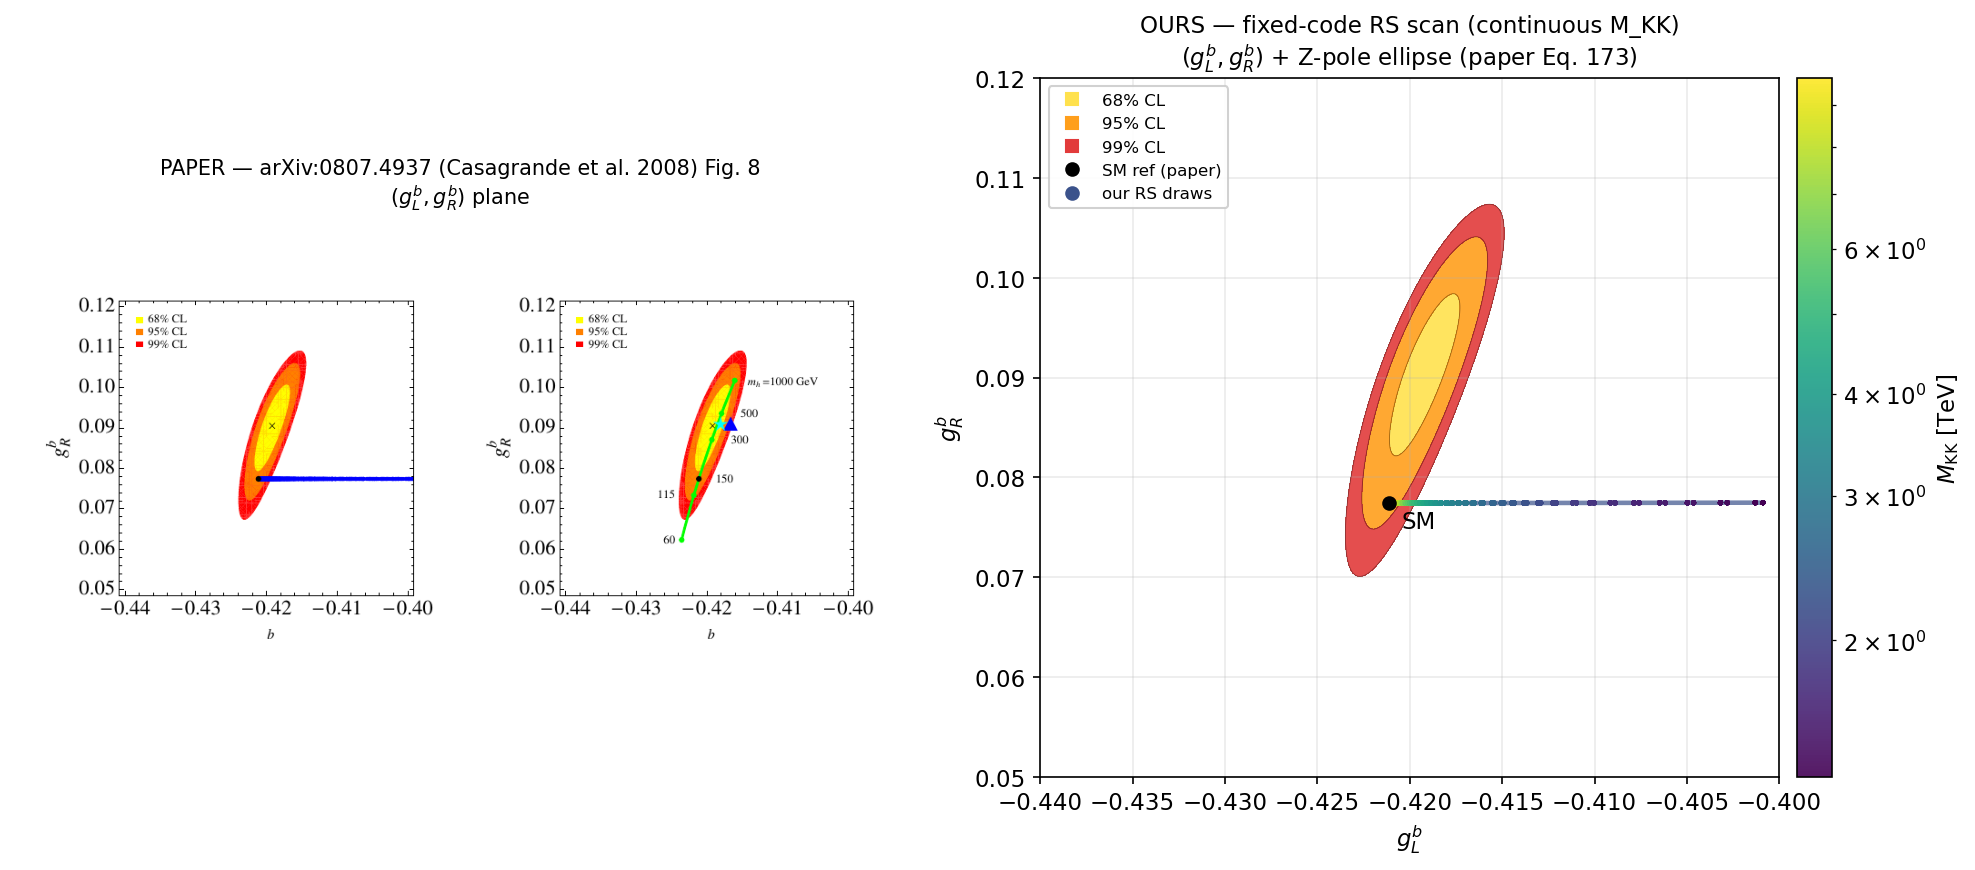
\includegraphics[width=\textwidth]{figures/fig_Zbb_gLgR.png}
\caption{The $(g_L^b, g_R^b)$ plane: paper (left) vs.\ ours (right), with the
$Z$-pole CL ellipses and the SM point.}
\end{figure}
The $(g_L^b, g_R^b)$ plane with the $Z$-pole CL ellipses and the SM point. We use
essentially the same $R_b/A_b$ as the paper, so the SM point and ellipses overlay
identically (the sanity check). With the \textbf{B1} fix, the \emph{total}
coupling shift $R_b$ sees --- gauge-KK (dominant, $+8.7\times10^{-5}$ at 20~TeV,
reproducing the audit on the nose) plus the corrected fermion admixture --- moves
$g_L^b$ to less-negative values as $M_{KK}$ drops, the CGHNP direction. The
original bug had the fermion piece wrong-sign and ${\sim}190\times$ too large,
faking a 25--30~TeV exclusion; corrected, $Z\to b\bar b$ is gauge-dominated and
bites only to ${\sim}5$~TeV.

\FloatBarrier

% ---- epsK_cloud ----
\subsection*{$\varepsilon_K$ --- Bauer et al.\ 0912.1625, Fig.~4 \quad(paper left, ours right)}
\begin{figure}[H]
\centering
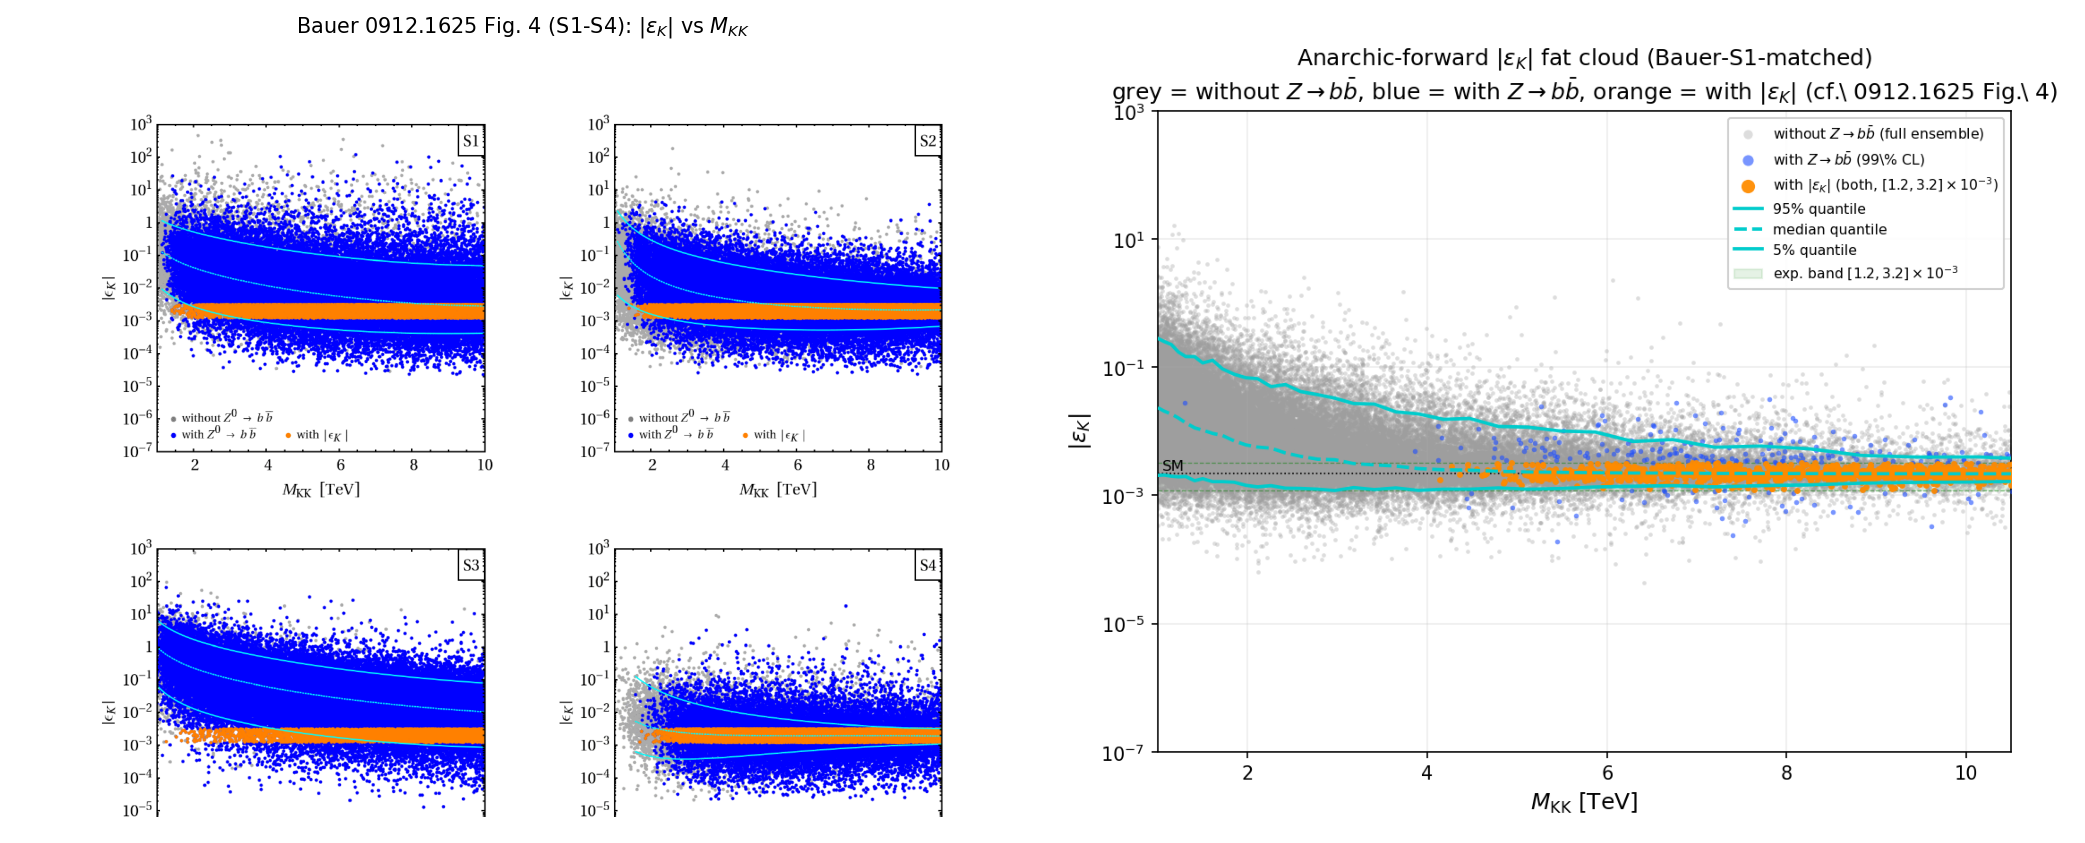
\includegraphics[width=\textwidth]{figures/fig_epsK_cloud.png}
\caption{Anarchic $|\varepsilon_K|$ vs.\ $M_{KK}$: paper (left, S1--S4) vs.\ ours
(right, S1), Bauer's grey/blue/orange $Z\to b\bar b$ colouring with 5/50/95\%
quantile curves. Paper scatters anarchic Yukawas; we reproduce the fat cloud in
anarchic-forward mode. Grey and the quantiles come from the fat 990k anarchic-S1
ensemble (restoring Bauer's tail spread); dense blue/orange from the 202k
$Z\to b\bar b$ companion --- both the same Bauer-S1 prior.}
\end{figure}
The canonical RS $\varepsilon_K$ problem: anarchic $|\varepsilon_K|$ vs.\
$M_{KK}$ spanning ${\sim}6$ decades, colored by $\varepsilon_K$ consistency, with
5/50/95\% quantile curves. The key methodological point: the paper
\textbf{scatters} anarchic $O(1)$ Yukawas (fat cloud) while our production scan
\textbf{fits} to masses+CKM (thin locus). We now run the fixed code in an
anarchic-forward mode that \textbf{matches Bauer's S1 draw setup}
(\texttt{scripts/anarchic\_bauer\_s1.py}): $|Y|$ uniform in modulus over
$[0.1,\,Y_{\max}=3]$ with uniform phase, and per-draw \textbf{scanned} bulk
masses (the RH-top $c_{u_3}$ flat in Bauer's prior; the rest fixed by the
leading-order Froggatt--Nielsen relations from the drawn Yukawa minors). This
reproduces the \textbf{per-tile ${\sim}6$-decade cloud} (was ${\sim}3.3$ with the
older fixed-$c$, $|Y|<2.1$ generator), the \textbf{95\%-quantile floor at
$M_{KK}\approx10$~TeV} (= Bauer's ``$M_g^{(1)}\gtrsim10$~TeV''), and the
upper-bulk amplitude ($p75\approx118\times$ SM = Bauer's ``typically
${\sim}100\times$ SM''). The fitted $c$'s land on Bauer's Table~1 central values.
The figure is a HYBRID of two layers from the SAME Bauer-S1 prior. The grey
backdrop and the 5/50/95\% quantiles come from the FAT 990{,}000-draw
\texttt{anarchic\_bauer\_S1} ensemble (112{,}024 mass+CKM-gated draws on the
45-tile 1--20~TeV grid), which samples the $|\varepsilon_K|$ tails far better than
the companion run and restores Bauer's headline per-tile spread (median ${\sim}3.7$,
max ${\sim}4.9$ decades). The dense blue ($Z\to b\bar b$-passing) and orange
($|\varepsilon_K|$-window) overlays come from the 202{,}500-draw
\texttt{anarchic\_bauer\_s1\_zbb} companion (22{,}880 mass+CKM-gated, 5{,}401
$Z\to b\bar b$-passing blue, ${\sim}5{,}000$ in-window orange). Both layers are the
same anarchic prior, so blue is a representative $Z\to b\bar b$-passing subset of the
grey distribution. One honest, real difference (not
a plotting artifact): our blue ($Z\to b\bar b$-consistent) points fill in only
ABOVE ${\sim}4.5$~TeV, whereas Bauer's blue blankets the plane down to 1~TeV ---
because our corrected $Z\to b\bar b$ (PDG-2025 $R_b/A_b$ + exact coupling) is
genuinely STRONGER than Bauer's 2009 version and vetoes low-$M_{KK}$ draws he would
have kept. The spread, floor, axes, colouring and scenario ordering all match. A
companion $2\times2$ S1--S4 panel mirrors the paper's full layout (S3
``little'' sits an order of magnitude higher from UV dominance, exactly as
published). With current (vs.\ paper-era) constraints the $\geq50\%$ floor rises
to ${\sim}30$~TeV.

\FloatBarrier

% ---- consistency ----
\subsection*{Consistency fraction --- Bauer et al.\ 0912.1625, Fig.~5 \quad(paper left, ours right)}
\begin{figure}[H]
\centering
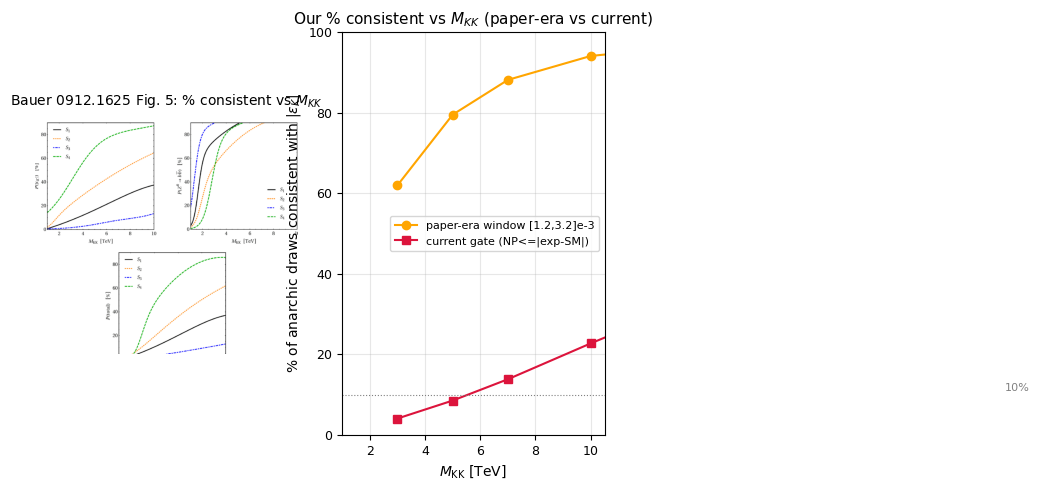
\includegraphics[width=\textwidth]{figures/fig_consistency.png}
\caption{Percentage of anarchic points consistent vs.\ $M_{KK}$: paper (left) vs.\
ours (right), for both paper-era and current inputs.}
\end{figure}
Percentage of anarchic points consistent vs.\ $M_{KK}$: a rising S-curve with
$1/M_{KK}^2$ decoupling, where $Z\to b\bar b$ consistency turns on before the
combined fraction. Ours reproduces the same ordering and decoupling, shown for
both paper-era and current inputs.

\FloatBarrier

% ---- CBd_phiBd ----
\subsection*{$B_d$ mixing --- Bauer et al.\ 0912.1625, Fig.~6 \quad(paper left, ours right)}
\begin{figure}[H]
\centering
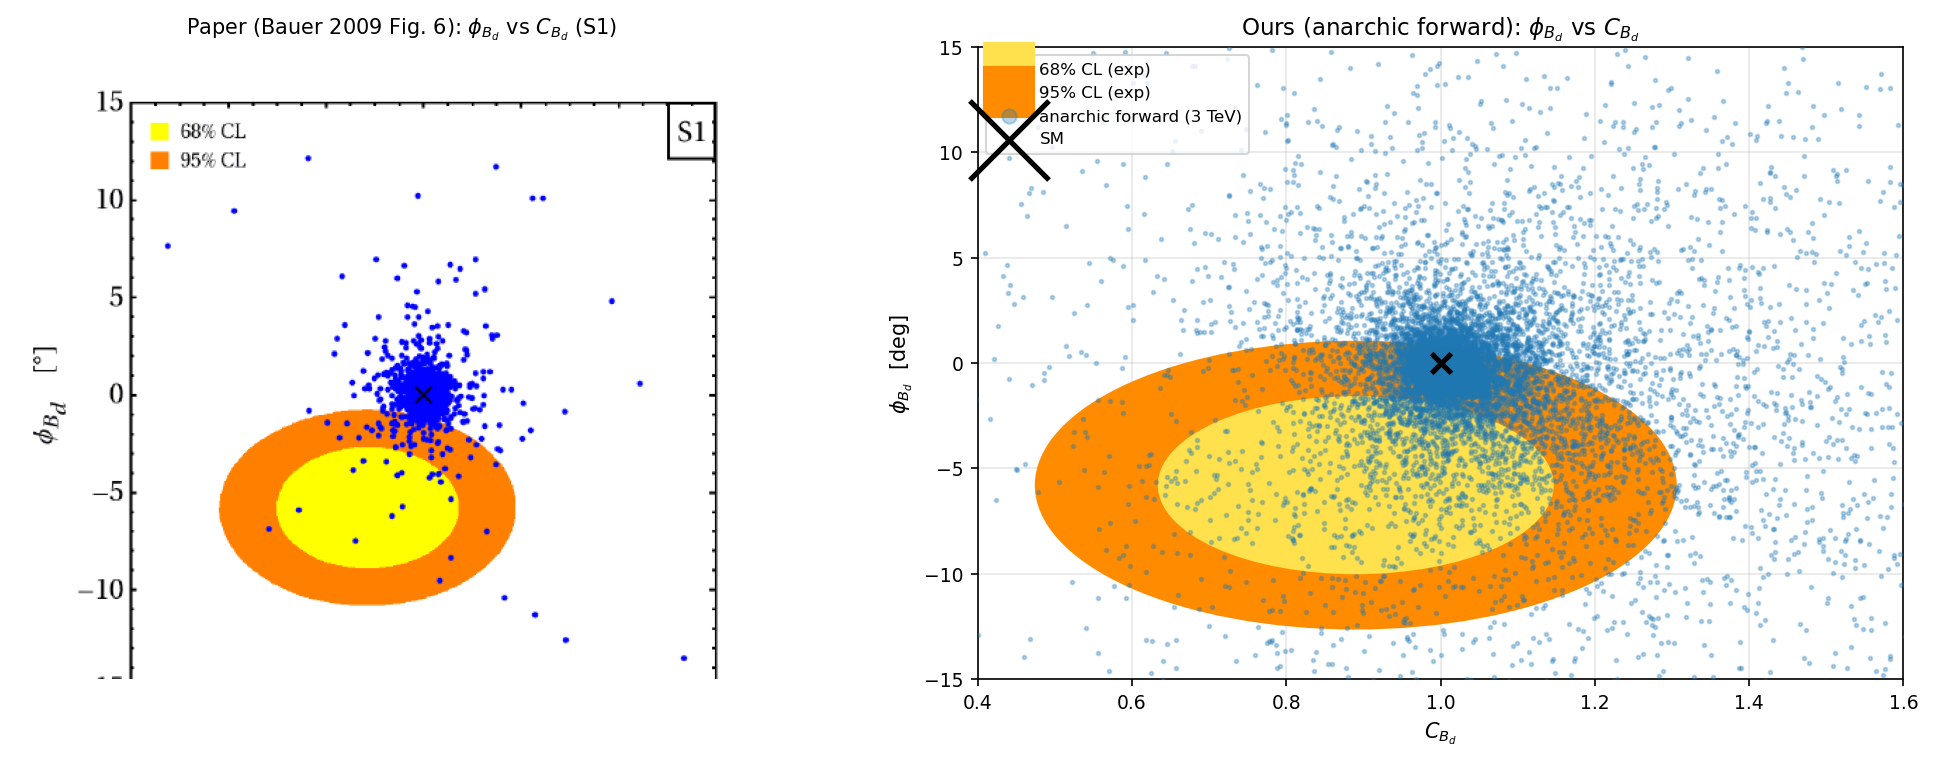
\includegraphics[width=\textwidth]{figures/fig_CBd_phiBd.png}
\caption{The $B_d$-mixing NP plane ($C_{B_d}$ vs.\ $\phi_{B_d}$): paper (left)
vs.\ ours (right), centered near the SM point $(1,0)$.}
\end{figure}
The $B_d$-mixing new-physics plane: amplitude $C_{B_d}$ vs.\ phase $\phi_{B_d}$.
Our anarchic model points (Bauer S1 ensemble, $Y_{\max}=3$, scanned $c$) cluster
near the SM point $(1,0)$ --- $C_{B_d}$ median $1.02$, $p5 = 0.89$ (= Bauer's
$C_{B_d} = 0.89\pm0.17$), $\phi_{B_d}$ a few degrees about $0$ --- exactly as
Bauer's blue scatter does. We now also overlay the same experimental $68/95\%$ CL
allowed ellipses the paper draws ($C_{B_d}=0.89\pm0.17$, $\phi_{B_d}=-5.8\pm2.8^\circ$);
our cloud sits within/around them just as in Fig.~6 (these were missing from the
earlier version, which is what made it not look like the paper).

\FloatBarrier

% ---- CBs_phiBs ----
\subsection*{$B_s$ mixing --- Bauer et al.\ 0912.1625, Fig.~7 \quad(paper left, ours right)}
\begin{figure}[H]
\centering
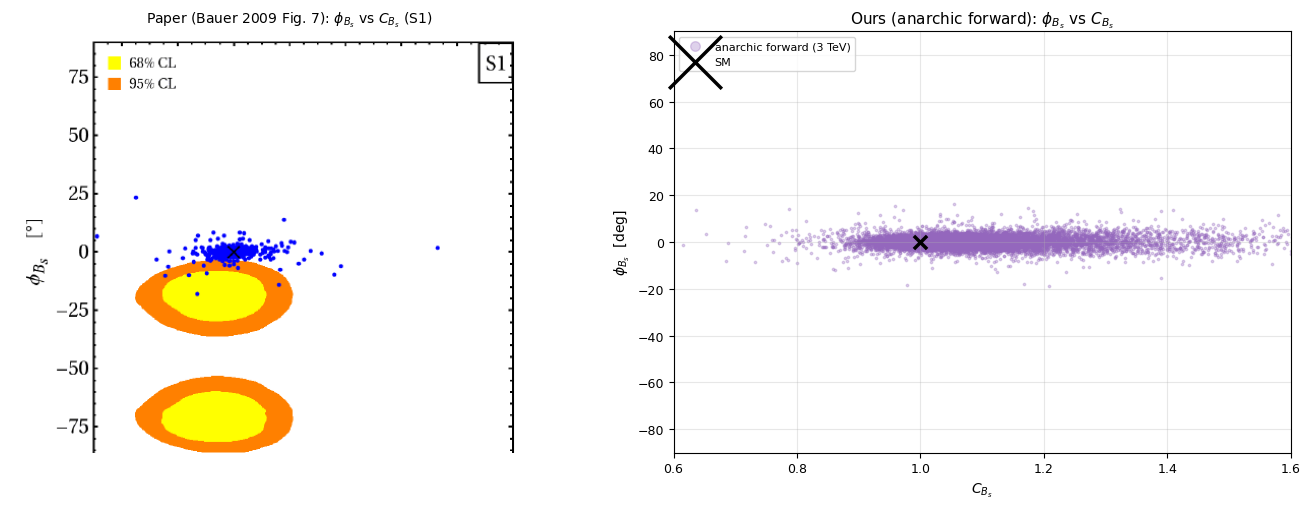
\includegraphics[width=\textwidth]{figures/fig_CBs_phiBs.png}
\caption{The analogous $B_s$ plane ($C_{B_s}$, $\phi_{B_s}$, $S_{\psi\phi}$):
paper (left) vs.\ ours (right).}
\end{figure}
The analogous $B_s$ plane. Our model points cluster near the SM point ($C_{B_s}$
median $1.04$, $p5 = 0.94$ = Bauer's $C_{B_s} = 0.93\pm0.19$); the $\phi_{B_s}$
scatter is \emph{narrow} ($\pm{\sim}20^\circ$), which correctly matches Bauer's own
model points --- the wide $\pm60$--$70^\circ$ features in the figure are the
\emph{experimental} twofold CL regions ($\phi_{B_s}\approx-19^\circ$ and
$-70^\circ$), which we now draw. The model $B_s$ phase is suppressed because
$|M_{12}^{\rm NP}|/|M_{12}^{\rm SM}|\approx0.1$ in the matched ensemble; the
amplitude $\arg(M_{12}^{\rm NP})$ itself is uniform, as it should be.

\FloatBarrier

% ---- D0_funnel ----
\subsection*{$D^0$ mixing --- Gedalia, Grossman, Nir, Perez 0906.1879, Fig.~1 \quad(paper left, ours right)}
\begin{figure}[H]
\centering
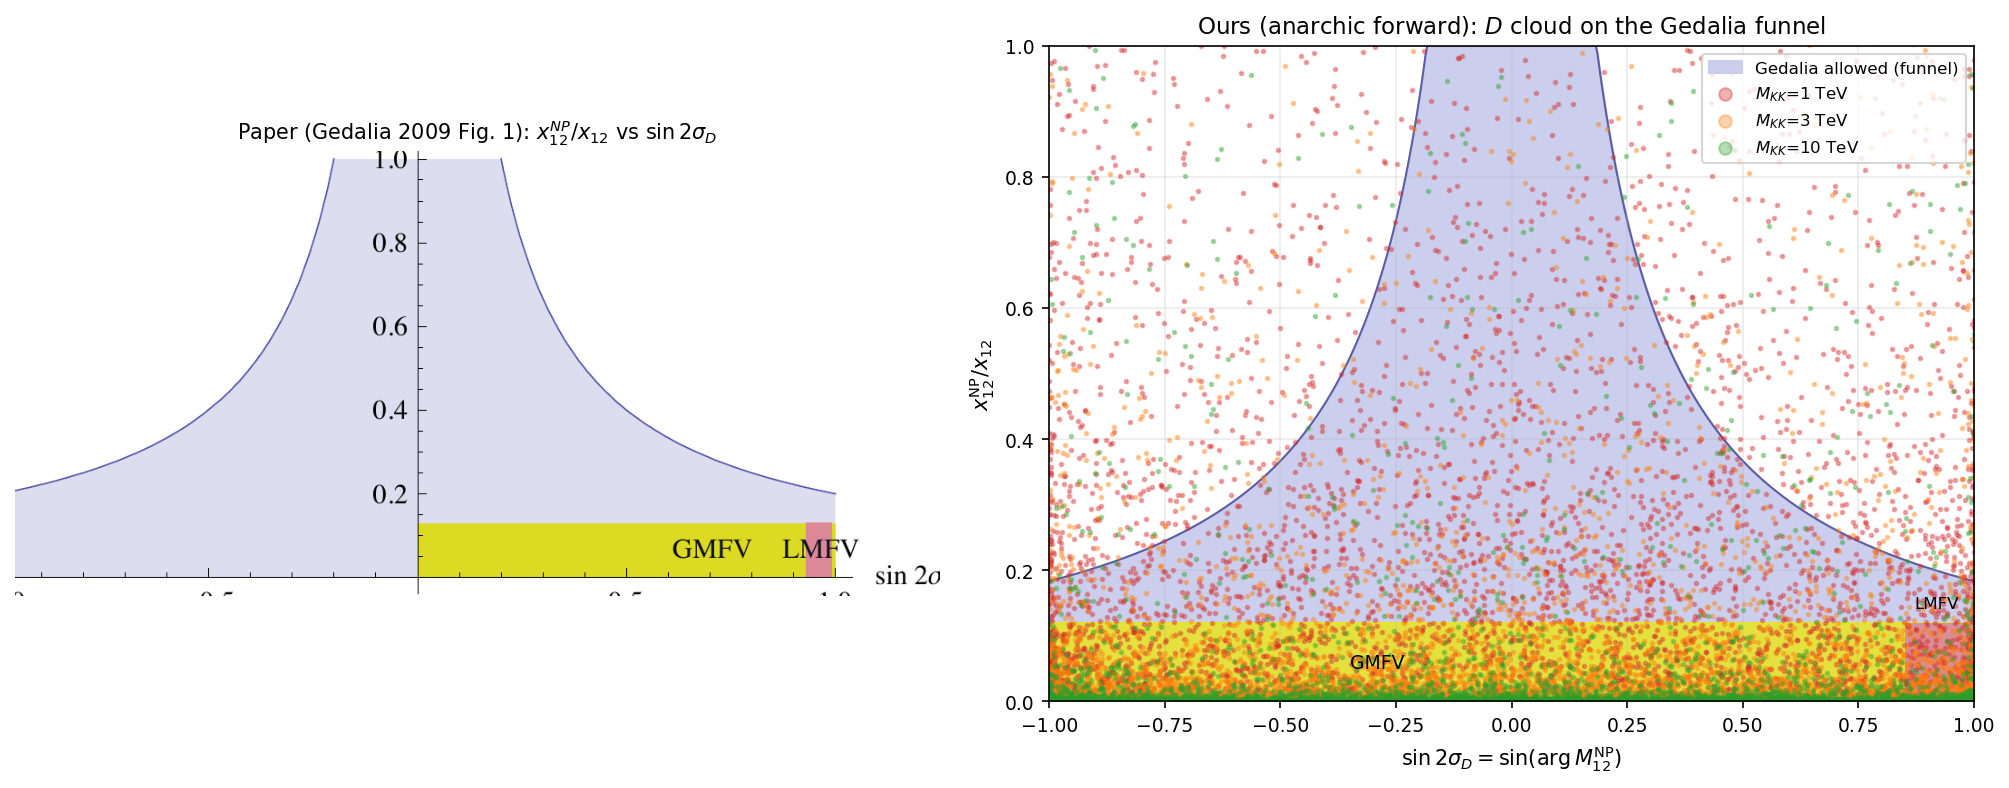
\includegraphics[width=\textwidth]{figures/fig_D0_funnel.png}
\caption{The allowed ``funnel'' in $(x_{12}^{\mathrm{NP}}/x,\ \sin2\sigma_D)$:
paper (left) vs.\ ours (right). Our cloud sinks into the allowed funnel as
$M_{KK}$ rises.}
\end{figure}
The allowed ``funnel'' in $(x_{12}^{\mathrm{NP}}/x,\ \sin 2\sigma_D)$. Our matched
anarchic $D$-meson cloud (carrying the complex $M_{12}$ phase) sinks into the grey
allowed funnel as $M_{KK}$ rises --- inside-funnel fraction 50\% at 1~TeV $\to$
77\% at 3~TeV $\to$ 88\% at 10~TeV --- a faithful reproduction (the wider matched
ensemble gives a broader, more paper-like cloud than the earlier fixed-$c$ run).

\FloatBarrier

% ---- ReIm_M12 ----
\subsection*{$\Delta F=2$ amplitudes --- Blanke et al.\ 0809.1073, Fig.~2 \quad(paper left, ours right)}
\begin{figure}[H]
\centering
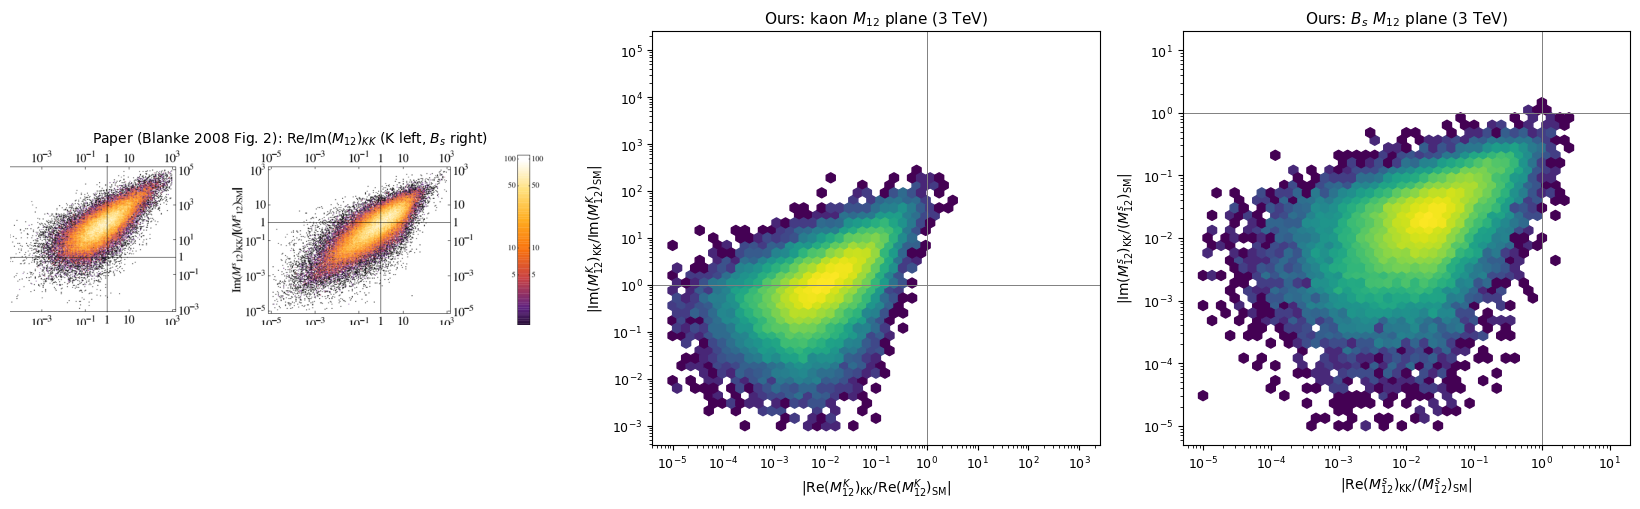
\includegraphics[width=\textwidth]{figures/fig_ReIm_M12.png}
\caption{$\mathrm{Re}/\mathrm{Im}$ of the KK contribution to $M_{12}$ for the $K$
and $B_s$ systems: paper (left) vs.\ ours (right).}
\end{figure}
$\mathrm{Re}/\mathrm{Im}$ of the KK contribution to $M_{12}$ for the $K$ and $B_s$
systems. For kaons, Blanke note $\mathrm{Im}(M_{12})\gg\mathrm{Re}$ by
${\sim}100\times$ (the $\varepsilon_K$ problem); \textbf{ours = 106$\times$}
(ratio of medians at 3~TeV). For $B_s$ the contribution is $O(1)$. Both reproduce
the paper.

\FloatBarrier

% ---- existence_vs_typical ----
\subsection*{Existence vs.\ typical floors (our analysis, ours only)}
\begin{figure}[H]
\centering
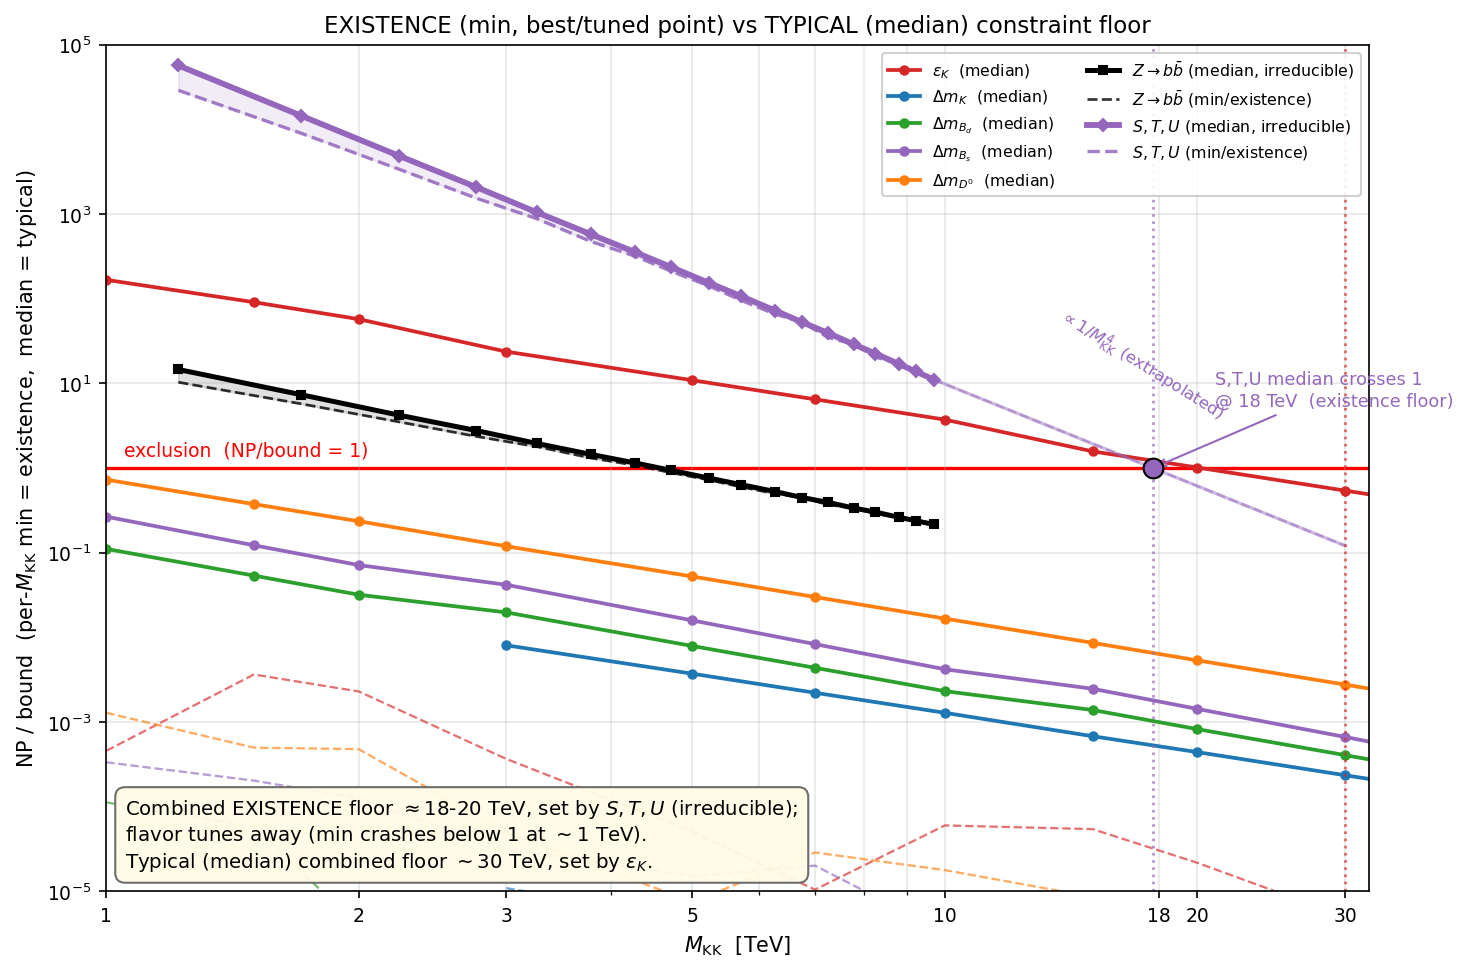
\includegraphics[width=\textwidth]{figures/fig_existence_vs_typical.png}
\caption{Per constraint: \textbf{minimum} ratio-to-bound (the best fine-tuned
point $\to$ existence floor) and \textbf{median} ratio (typical anarchic point)
vs.\ $M_{KK}$.}
\end{figure}
For each constraint we plot the \textbf{minimum} ratio-to-bound (the best,
fine-tuned point $\to$ the \emph{existence} floor) and the \textbf{median} ratio
(the \emph{typical} anarchic point) vs.\ $M_{KK}$. The flavor constraints
($\varepsilon_K$, $\Delta m_d$, $\Delta m_s$, $D^0$, $\Delta m_K$) are fully
\textbf{tunable}: even at 1~TeV the best point beats the bound by ${\sim}1000\times$
(alignment sends $\varepsilon_K\propto\mathrm{Im}\,M_{12}\to0$), so their
existence floor is ${\lesssim}1$~TeV. \textbf{$S,T,U$ is irreducible} ---
min $\approx$ median (spread only ${\sim}1.5\times$) because it has no Yukawa
dependence --- crossing the bound only at ${\sim}18\text{--}20$~TeV. Hence even
with maximally fine-tuned Yukawas, minimal RS cannot exist below
${\sim}18\text{--}20$~TeV, set by oblique $S,T,U$; $Z\to b\bar b$ is the next
irreducible one at ${\sim}4.6$~TeV.

\FloatBarrier
\clearpage

% ===================== CONCLUSION =====================
\section{Conclusion}

The fixed, dual-reviewed code reproduces the published RS flavor/EWPT literature
across seven figures from four papers, matching their quoted numbers
($\varepsilon_K$ 10~TeV floor, $D^0$ containment, kaon $100\times$ $\varepsilon_K$
problem, $C_{B_d}/C_{B_s}\approx1$). The corrected minimal-model picture: the
\emph{typical} anarchic floor with current data is ${\sim}30$~TeV, dominated by
the (tunable) $\varepsilon_K$ constraint; the \emph{existence} floor for a
fine-tuned point is ${\sim}18\text{--}20$~TeV, dominated by the (irreducible)
$S,T,U$ oblique constraint. The earlier 25--30~TeV $Z\to b\bar b$ ``floor'' was a
sign-bug artifact (now 5~TeV). Pushing below ${\sim}20$~TeV requires custodial
protection of $T$ (custodial RS), which is the next branch of this program.

\end{document}
